% Kelompok 2 Tugas 2 GIS (DATA RASTER)
% Tiara Rizki Wulansari (1154026)
% Muhamad Rifan Zamaludin (1154088)
% Mohammad Agung Deomartha (1154032)
% M. Fajri Mualim (1154078)
% Faisal Syarifuddin (1154104)

\section{Data Raster}
\subsection{Pengertian Data Raster}
Data raster \cite{puntodewo2003sistem} adalah data yang disimpan dalam bentuk kotak segi empat (grid) sel sehingga terbentuk suatu ruang yang 
teratur. Foto digital seperti areal fotografi atau satelit merupakan bagian dari data raster pada peta. 
Raster memiliki data grid continue. Nilainya menggunakan gambar berwarna seperti fotografi, yang ditampilkan dengan 
level merah, hijau, dan biru pada sel. Data Raster (atau disebut juga dengan sel grid) merupakan data yang 
dihasilkan dari sistem penginderaan jauh. Pada data raster. Obyek geografis direpresentasikan sebagai struktur
sel grid yang disebut dengan pixel (picture element). Pada data raster. Resolusi (definisi visual) tergantung
pada ukuran pixelnya. Dengan kata lain. Resolusi pixel menggambarkan ukuran sebenarnya dipermukaan bumi 
yang diwakili oleh setiap pixel pada citra. Pada data raster, Obyek geografis direpresentaskan sebagai struktur sel grid yang disebut sebagi pixel (picture element). Resolusi (definisi visual) tergantung pada ukuran pixel-nya, semakin kecil ukuran permukaan bumi yang direpresentasikan oleh sel, semakin tinggi resolusinya. Data Raster dihasilkan dari sistem penginderaan jauh dan sangat baik untuk merepresentasikan batas-batas yang berubah secara gradual seperti jenis tanah, kelembaban tanah, suhu, dan lain-lain. Peta raster adalah peta yang diperoleh dari fotografi suatu areal. foto satelit atau foto permukaan bumi yang diperoleh dari komputer. Contoh peta raster yang diambil dari satelit cuaca. Di dalam Sig, data raster dan analisis data raster banyak digunakan untuk pemetaan obyek yang bersifat kontinu (batasnya tidak terlihat jelas di lapangan/gradual) dan pemodelan spasial, baik statis maupun dinamis. Analisis data raster banyak menggunakan peta-peta hasil analisa digital citra satelit karena peta raster dan citra satelit mempunyai struktur data yang sama, yaitu grid cell, sehingga kompatibel satu degan yang lain. Hal ini berbeda dengan data vector, dimana agar bisa dianalisis secara bersama, Data raster hasil analisis harus dikonversi dulu ke struktur data vektor \cite{puntodewo2003sistem}.

\subsection{Pengertian Data Vektor}
Data vektor adalah data yang direkam dalam bentuk koordinat titik yang menampilkan, 
menempatkan dan menyimpan data spasial dengan menggunakan titik, 
garis atau area (polygon). Ada tiga tipe data vector (titik, garis, 
dan polygon) yang bisa digunakan untuk menampilkan informasi pada peta. 
Titik bisa digunakan sebagai lokasi sebuah kota atau posisi tower radio. 
Garis bisa digunakan untuk menunjukkan route suatu perjalanan atau menggambarkan boundary. 
Poligon bisa digunakan untuk menggambarkan sebuah danau atau sebuah Negara pada peta dunia.

\subsection{Kelebihan dan kekurangan Data Raster}
\subsubsection{Kelebihan Data Raster}
Adapun kelebihan yang dimiliki oleh data raster menurut \cite{irwansyah2013sistem} adalah: 
	\begin{enumerate}
		\item memiliki struktur data yang sederhana
		\item mudah dimanipulasi dengan menggunakan fungsi-fungsi matematis sederhana
		\item teknologi yang digunakan cukup murah dan tidak begitu kompleks sehingga pengguna dapat membuat sendiri program aplikasi yang menggunakan citra raster
		\item compatible dengan citra-citra satelit penginderaan jauh dan semua image hasil scanning data spasial.
		\item Overlay dan kombinasi data raster dengan data inderaja mudah dilakukan.
		\item memiliki kemampuan-kemampuan pemodelan dan analisis  spasial tingkat lanjut.
		\item metode untuk mendapatkan citra raster lebih mudah
		\item Gambar permukaan bui dalam bentuk citra raster yang didapat dari radar atau satelit penginderaan jauh selalu aktual dari pada bentuk vektornya
		\item prosedur untuk emperoleh data dalam bentuk raster lebh mudah, sederhana dan murah.
		\item Harga sistem perangkat lunak aplikasinya cenderung lebih murah.
	\end{enumerate}

\subsubsection{Kekurangan Data Raster}
Adapun Kekurangan yang dimiliki oleh data raster menurut \cite{irwansyah2013sistem} adalah :
	\begin{enumerate}
		\item secara umum memerlukan ruang atau tempat penyimpanan (disk) yang besar dalam komputer, banyak terjadi redudancy data baik untuk setiap layer-nya maupun secara keselururhan.
		\item Pengunaan sel atau ukuran grid yang lebih besar untuk menghemat ruang penyimpaanan akan menyebabkan kehilanagn informasi dan ketelitian.
		\item sebuah citra raster hanya mengandung satu tematik saja sehingga sulit digabungkan dengan atribut-atribut lainnya dalam satu layer.
		\item tampilan atau reprsentasi dan akurasi posisi sangat bergantung pada ukuran pikselnya (resolusi spasial)
		\item sering mengalami kesalahan dalam menggambarkan bentuk dan garis batas suatu obyek. sangat bergantung pada resolusi spasial dan toleransi yang diberikan
		\item transformasi koordinat dan proyeksi lebih sult dilakukan
		\item sangant sulit untuk mepresentasikan hubungan topologi (juga network)
		\item metode untuk medapatakan format data vektor melalui proses yang lama, cukup melelahkan dan relative mahal.
	\end{enumerate}

\subsection{perbedaan data raster dan data vektor}
Masing-masing format data mempunyai kelebihan dan kekurangan.
Pemilihan format data yang digunakan sangat tergantung pada tujuan penggunaan. 
Data yang tersedia, volume data yang dihasilkan, ketelitian yang diinginkan, serta kemudahan dalam Analisa.

Data Vektor relatif lebih ekonomis dalam hal ukuran file dan presisi dalam lokasi. Tetapi sangat sulit untuk 
digunakan dalam komputasi matematik.
Sebaliknya Data raster biasanya membutuhkan ruang pentyimpanan file yang lebih besar dan presisi lokasinya lebih rendah.
Tetapi lebih mudah digunakan secara matematis.
Model data raster mempunyai struktur data yang tersusun dalam bentuk matriks atau pixel dan membentuk grid. 
Setiap pixel memiliki nilai tertentu dan memiliki atribut tersendiri, termasuk nilai kordinat yang unik.

Tingkat keakurasian model ini sangat tergantung pada ukurasn piksel atau biasa disebut resolusi.
Model data ini biasanya digunakan dalam remote sensing yang berbasiskan citra satelit maupun airborn (pesawat terbang).
Selain itu model ini digunakan pula dalam membangun model ketinggian digital(DEM-Digital Elevation Model) dan model permukaan digital(DTM-Digital Terrain Model).
Model Raster Memberikan Informasi spasial terhadap permukaan di bumi dalam bentuk gambaran yang digeneralisasi.
Represantasi dunia nyata disajikan sebagai elemen matriks atau piksel yang membentuk grid  yang homogen. 
Pada setiap piksel mewakili setiap obyek yang terekam dan ditandai dengan nilai-nilai tertentu.
Secara konseptual model data raster merupakan model data spasial yang paling sederhana. 

\subsection{karakteristik data raster}
Resolusi suatu data raster akan merujuk pada ukunan permukaan bumi yang direpresentasikan oleh setiap piksel. 
Makin kecil ukuran atau luas permukaan bumi yang dapat direpresentasikan oleh setiap pikselnya, 
makin tinggi resolusi spasialnya.
Piksel-piksel di dalam zone atau area yang sejenis memiliki nilai (isi piksel atau ID number) yang sama. 
Pada umumnya, lokasi di dalam model data raster, diidentifikasi dengan menggunakan pasangan koordinat kolom dan baris (x,y).

\subsection{Metode Penyimpanan Data Raster}
Data raster mempunyai beberapa metode penyimpanan data yaitu run length encoding, block encoding, chain encoding dan quadtree data structure.
	\begin{itemize}
		\item  Run Length Encoding
				mengurangi jumlah data pada setiap baris.
				\begin{figure} [ht]
					\centerline{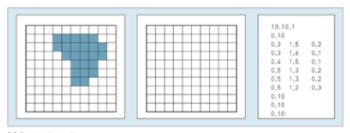
\includegraphics[width=1\textwidth]{figures/runlengthencoding.JPG}}
					\caption{Gambar Run Length Encoding}
					\label{runlengthencoding}
					Gambar \ref{runlengthencoding} adalah contoh gambar pada Run Length Encoding
				\end{figure}

		\item  Block Encoding
				metode ini memperluas dari Run Length encoding menggunakan rangkaian blok untuk menyimpan data.
				\begin{figure} [ht]
					\centerline{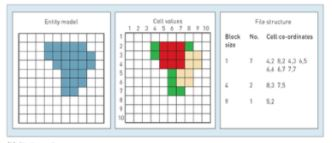
\includegraphics[width=1\textwidth]{figures/blockencoding.JPG}}
					\caption{Gambar Block Encoding}
					\label{blockencoding}
					Gambar \ref{blockencoding} adalah contoh gambar Block Encoding
				\end{figure}

		\item  Chain Encoding
				pengurangan data dengan mendefinisikan batas-batas entitas.
				\begin{figure} [ht]
					\centerline{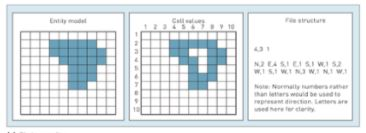
\includegraphics[width=1\textwidth]{figures/chainencoding.JPG}}
					\caption{Gambar Chain Encoding}
					\label{chainencoding}
					Gambar \ref{chainencoding} adalah contoh gambar pada Chain Encoding
				\end{figure}

		\item  Quadtree Data Structure
				Membagi setap sel dalam image ke dalam empat per empat bagian lalu dibagi lagi ke dalam kelas-kelas.
				\begin{figure} [ht]
					\centerline{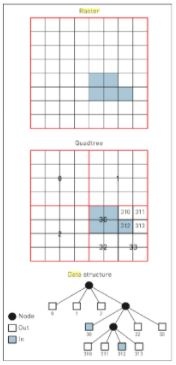
\includegraphics[width=0.25\textwidth]{figures/quadtreedatastructure.JPG}}
					\caption{Gambar Quadtree Data Structure}
					\label{quadtreedatastructure}
					Gambar \ref{quadtreedatastructure} adalah contoh gambar Quadtree Data Structure
				\end{figure}
	\end{itemize}

\subsection{Akses ikonik ke repositori format data raster data monokrom elektronik jarak jauh}
Dalam Akses ikonik ke repositori format data raster data monokrom elektronik jarak jauh, 
Dokumen disimpan dalam sistem menggunakan monokrom, format raster. 
Dokumen dikirimkan dari repositori ke situs akses jarak jauh untuk ditampilkan kepada pengguna. 
Kemampuan tambahan disediakan untuk mencari dokumen yang tersimpan; 
menghasilkan layar antarmuka pengguna sesuai permintaan yang berisi hasil pencarian; 
memasukkan dokumen ke dalam repositori via transmisi oleh mesin faksimili; 
dan untuk berkomunikasi secara interaktif antara pengguna sistem. 
Dokumen elektronik bisa berupa teks dan grafis konvensional; 
atau dokumen multi media yang berisi teks, video, dan materi audio. 
Sebuah repositori dokumen fisik tunggal dapat secara logis tersegmentasi menjadi
beberapa repositori virtual yang mendukung beragam kelompok pengguna.

\subsection{Pengertian PostGIS}
Sistem Informasi Geografis (SIG) adalah sistem informasi khusus yang mengelola data yang memiliki informasi spasial (bereferensi keruangan). 
Atau dalam arti sempit, adalah sistem komputer yang memiliki kemampuan untuk membangun,
menyimpan, mengelola dan menampilkan informasi bereferensi geografis, misalnya data yang diidentifikasi menurut lokasinya, dalam sebuah database.
SIG juga merupakan sejenis perangkat lunak, perangkat keras (manusia, prosedur, basis data) yang berguna untuk proses pemasukan, penyimpanan, menampilkan data geografis serta atribut-atribut yang terkait.
PostGIS adalah extender database spasial gratis untuk PostgreSQL, 
setiap bit sebaik perangkat lunak berpemilik. Dengan itu, 
Anda dapat dengan mudah membuat query dengan sadar lokasi hanya dalam beberapa baris kode SQL 
dan membangun bagian belakang untuk pemetaan, analisis raster, 
atau aplikasi perutean dengan sedikit usaha. 
PostGIS dalam Tindakan, mengajarkan untuk memecahkan masalah real- 
masalah geodata dunia Ini pertama memberi Anda latar belakang GIS vektor,
raster, dan topologi berbasis GIS dan kemudian dengan cepat bergerak 
untuk menganalisis, melihat, dan memetakan data.

\subsection{Uraian EMBODIMEN Yang Dimiliki}
Saat ini, cara terbaik untuk mempraktikkan penemuan ini adalah menerapkan sistem yang
menggunakan Internet sebagai General Purpose Data Network, 101, dalam gambar. 
Internet adalah Wide Area Network (WAN) yang terkenal dan mudah diakses. 
Sub-sistem Dokumen Repositori, 102, terdiri dari satu atau lebih sistem komputer fisik yang terhubung ke Internet. Sub-sistem Remote Access, 104, adalah sistem komputer individual dengan koneksi dedicated atau dial-up ke Internet.
Rincian Sub-dokumen Document Repository akan dibahas dengan mengacu pada Gbr. 2, 
kecuali Gambar lain secara khusus dirujuk. Document Repository secara logis tersegmentasi menjadi beberapa repositori virtual. 
Setiap repositori virtual khusus untuk pengguna atau kumpulan pengguna. Jelas, mekanisme keamanan lainnya juga berlaku. Pendekatan ini memberi pengguna tampilan repositori yang berdiri sendiri dan berdiri sendiri sambil menghindari biaya komputer dan perangkat keras dan pendukung yang berdedikasi. Setiap repositori virtual mendukung beberapa sesi bersamaan dengan Remote Access Sub-systems. 
Jumlah sesi tidak dibatasi oleh sejumlah port dial-in fisik di repositori. Dua tingkat keamanan disediakan untuk repositori. Yang pertama mencegah akses tidak sah ke repositori itu sendiri. Kontrol kedua mengakses repositori virtual tertentu.
